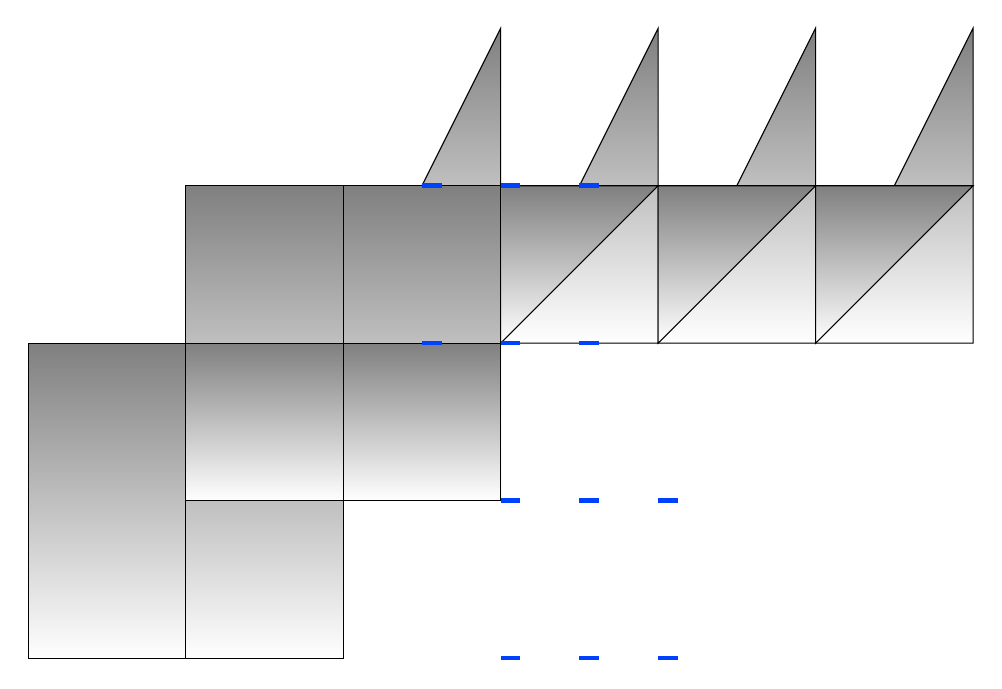
\begin{tikzpicture}[scale=1]

\shade[draw=black,fill=red!20] (-4,-4) -- (-2,-4) -- (-2,0) -- cycle;
\shade[draw=black,fill=red!20] (-2,-4) -- (0,-4) -- (0,0) -- cycle;
\shade[draw=black,fill=red!20] (0,-4) -- (2,-4) -- (2,0) -- cycle;
\shade[draw=black,fill=red!20] (2,-4) -- (4,-4) -- (4,0) -- cycle;
\shade[draw=black,fill=red!20] (-4,-4) -- (-4,-2) -- (-2,-2) -- cycle;
\shade[draw=black,fill=red!20] (-2,-4) -- (-2,-2) -- (0,-2) -- cycle;
\shade[draw=black,fill=red!20] (0,-4) -- (0,-2) -- (2,-2) -- cycle;
\shade[draw=black,fill=red!20] (2,-4) -- (2,-2) -- (4,-2) -- cycle;

\shade[draw=black,fill=red!20] (-6,-6) -- (-4,-6) -- (-4,-2) -- (-6,-2) -- cycle;
\shade[draw=black,fill=red!20] (-4,-6) -- (-2,-6) -- (-2,-2) -- (-4,-2) -- cycle;
\shade[draw=black,fill=red!20] (-2,-6) -- (-2,-4) -- (-2,-2) -- cycle;
\shade[draw=black,fill=red!20] (-6,-6) -- (-4,-6) -- (-4,-4) -- (-6,-4) -- cycle;
\shade[draw=black,fill=red!20] (-4,-6) -- (-2,-6) -- (-2,-4) -- (-4,-4) -- cycle;
\shade[draw=black,fill=red!20] (-2,-6) -- (-2,-4) -- (-2,-2) -- (-2,-4) -- cycle;

\shade[draw=black,fill=red!20] (-8,-8) -- (-6,-8) -- (-6,-6) -- (-8,-6) -- cycle;
\shade[draw=black,fill=red!20] (-6,-8) -- (-4,-8) -- (-4,-6) -- (-6,-6) -- cycle;
\shade[draw=black,fill=red!20] (-4,-8) -- (-4,-6) -- (-2,-6) -- (-4,-6) -- cycle;
\shade[draw=black,fill=red!20] (-8,-8) -- (-6,-8) -- (-6,-4) -- (-8,-4) -- cycle;
\shade[draw=black,fill=red!20] (-6,-8) -- (-4,-8) -- (-4,-4) -- (-6,-4) -- cycle;
\shade[draw=black,fill=red!20] (-4,-8) -- (-4,-6) -- (-2,-6) -- (-4,-6) -- cycle;
\shade[draw=black,fill=red!20] (-6,-6) -- (-4,-6) -- (-4,-4) -- (-6,-4) -- cycle;
\shade[draw=black,fill=red!20] (-4,-6) -- (-2,-6) -- (-2,-4) -- (-4,-4) -- cycle;
\shade[draw=black,fill=red!20] (-2,-6) -- (-2,-4) -- (-2,-2) -- (-2,-4) -- cycle;

\foreach \n in {-3,...,-1} {
  \draw[blue!75!cyan,ultra thick] (\n,-2) -- ++(right:0.25);
}

\foreach \n in {-3,...,-1} {
  \draw[blue!75!cyan,ultra thick] (\n,-4) -- ++(right:0.25);
}

\foreach \n in {-2,...,0} {
  \draw[blue!75!cyan,ultra thick] (\n,-6) -- ++(right:0.25);
}

\foreach \n in {-2,...,0} {
  \draw[blue!75!cyan,ultra thick] (\n,-8) -- ++(right:0.25);
}

\end{tikzpicture}